\documentclass{jsarticle}
\usepackage[dvipdfmx]{graphicx}
\usepackage{listings,jlisting}
\usepackage{float}

\title{情報工学実験1数理計画法}

\author{学生番号4617043 神保光洋}
\date{\today}
\begin{document}
\maketitle
\section{実験目的}
本実験では非線形計画問題に対する基本的な解法である最急降下法、ニュートン法、
準ニュートン法
の実装とさまざまな問題への適用を通し、
アルゴリズムの特性の把握の大切さを学ぶことを目的とする

\section{アルゴリズムと数学的理論についての概要}
\subsection{無制約最小化問題に対する基礎理論}
無制約最小化問題とは、n変数関数 f: $R^2$ -> $R$ に対して定義される
以下の方法である。
最小化
$\{ f(x) | x = (x_1, x_2, x_3, ..., x_n) \} \in R^n$ 略して $\min{x \in R^n} f(x)$

\subsubsection{諸定義}
\paragraph{関数の勾配ベクトル、ヘッセ行列、テイラー展開}
$n$変数関数 $f : R^n \rightarrow R$ に対し、勾配ベクトル $\nabla f(x)$
とヘッセ行列 $\nabla^2 f(x)$ はそれぞれ以下のように定義されるベクトルと行列である。

$$
\nabla f(x) =
\begin{pmatrix} 2 \\ 2 \end{pmatrix}
$$

勾配ベクトルとヘッセ行列はそれぞれ一変数関数$f(x)$の微分係数と2階微分係数$f'(x)$
をn変数関数にしたものである。
なお、微分できない一変数関数もあるのと同様に、勾配ベクトルやヘッセ行列が定義できない関数
(f(x) = max($x^Tx, 0)$)
になることに注意する。
$f(x)$ が2階微分可能であれば、勾配ベクトルとヘッセ行列を用いて$x=a$において、
以下の式で$f(x)$を2次近似することができる($x=a$に置ける周りのテイラー展開を2次の項まで
求めたもの)。
\\
$ f(a + d) = f(a) + \nabla f(x)^Td + \frac{1}{2}d^T\nabla^2f(a)d + $ 残差

行列の正定値性
$n \times n$ 対称行列$X$が半正定値であるとは

$$
d^TXd \geq 0 \forall d \in R^n
$$

$n \times n$ 対称行列$X$が正定値であるとは \\
$d^TXd \geq 0 \forall d \in R^n$,$d \neq 0$

$n \times n$対称行列$X$が半正定値(正定値)であることと、$X$の固有値が全て非負(正)であること
は同値である。

\subsubsection{最適解と最適性条件}
\paragraph{最適解} 問題$\min{x \in R^n} f(x)$において、目的関数$f$を最小にする
$x^{\ast} \in R^n$, すなわち

$$
f(x^{\ast}) leq f(x) \forall \in R^n
$$

を満たす$x^{\ast}$を最適解と呼ぶ。最適解は次に定義する局所的最適解と区別するために大域的最適解
と呼ぶことも多い。

\paragraph{局所最適解} $x^{\ast}$を中心とする(小さな)球の中で目的関数$f$ を最小にする $x^{\ast} \in R^n :$ \\
ある$\epsilon > 0$ が存在して \\

$f(x^{\ast}) \leq f(x)$   $\forall x \in R^n$, $|| x^{\ast} - x || < \epsilon$ \\

を局所的最適解と呼ぶ。大域的最適解は局所的最適解になっているが、逆は成り立たない

一般に非線形最適化問題において大域的最適解を求めることは大変難しく、多くの場合は局所的最適解を求めることを
目指す。局所最適解については以下の最適性条件が成り立つ。

\paragraph{最適性条件}
\subparagraph{最適性の必要条件} $x^{\ast} \in R^n$ を局所的最適解とする。

\begin{itemize}
  \item $f$ が連続的微分可能 $\rightarrow \nabla f(x^{\ast}) = 0$ (1次の必要条件)。
  \item $f$が2階連続的微分可能 $\rightarrow {\nabla}^2 f(x^{\ast})$ 半正定値行列 (2次の必要条件)。
\end{itemize}

\subparagraph{2次の十分条件}
関数$f$が2階連続的微分可能とする。$x^{\ast} \in R^n$ が以下の条件
を満たすならば局所的最適解である。
\begin{description}
  \item $\nabla f(x^{\ast}) = 0$
  \item ${\nabla}^2 f(x^{\ast})$ が正定値行列
\end{description}

なお、1次の必要条件$\nabla f(^{\ast}) = 0$を満たす$x^{\ast}$ を停留点と呼ぶ。


\paragraph{凸関数}
関数 $f:R^n \rightarrow R$ が以下の条件を満たす時、凸関数であるという。

$$
f(\lambda x + (1 - \lambda)y) \leq \lambda f(x) + (1 - \lambda) f(y) {\forall}x , y \in R^n
$$

$f$が2階連続的微分可能であるとき、以下の事実が成り立つ。\\

$f$ が凸関数 $\iff {\nabla}^2 f(x)$ が半正定値行列 $\forall x \in R^n$

さらに、凸関数は次の「局所最適性=大域的最適性」を満たす。\\

fが凸関数のとき、$x^{\ast}$が$f$の局所的最適解 $\Rightarrow x^{\ast}$は$f$の大域的最適解
これより、微分可能な凸関数に対しては、$\nabla f(x) = 0$ を満たす $x^{\ast}$を求めれば、
その$x^{\ast}$は
最適解であることが保証される。このように、大域的最適解が必ず求まる関数のクラスとして、
凸関数は重要なクラスである

\subsubsection{反復法}
適当な初期点 $x_0 \in R^n$ からスタートし、以下の更新式で次々と点$x_1, x_2, \ldots$ を生成する
アルゴリズムを反復法という。

$$
x_{k+1} = x_k + {\alpha}_k d_k
$$

この式に置ける$d_k$を探索方向、$\alpha_k$をステップ幅という。探索方向は次で定義する降下方向に
なっているものを選び、ステップ幅は直線探索を利用して求めることが多い。
\paragraph{降下方向}
$x \in R^n$ における降下方向とは以下の条件を満たす$d \in R^n$ であり、
目的関数値が減少する方向である。
$\nabla f(x)^Td < 0$

\paragraph{最急降下方向}
$\nabla f(x) \neq 0$ であれば、$-\nabla f(x)$ は自明な降下方向である。
これを最急降下方向という。

\paragraph{直線探索を用いた反復法}

\begin{description}
  \item[ステップ0:] 初期点$x_0$を選び、$k := 0$とする
  \item[ステップ1:] 停止条件が満たされていれば終了する
  \item[ステップ2:] 探索方向$d_k$を定める
  \item[ステップ3:] 直線探索を用いてステップ幅${\alpha}_k$を定める
  \item[ステップ4:] $x_{k+1} := x_{k} + {\alpha}_kd_k, k := k + 1$としてステップ1に戻る
\end{description}

停止条件は、勾配ベクトルの大きさ$||\nabla f(x_k)||$が十分小さくなったことなど
に設定することが多い。

\subsubsection{直線探索}
点$x_k \in R^n$ と $x_k$における降下方向$d_k$が与えられたときに可能ならばステップ幅${\alpha}$を

$$
f(x_k + {\alpha}_kd_k) = \min \{f(x_k + \alpha d_k)  | \alpha > 0\}
$$

となるように選びたい。関数$f$が凸2次関数の場合は陽な値として正確に${\alpha}_k$が
求まるが、そうでなければこの問題は非常に難しい(それ自体が一変数の最小化問題)。
多くの場合は次のアルミホ条件を満たすように${\alpha}_k$を求める。\\

\subparagraph{アルミホ条件}
$0 < \xi < 1$を満たす定数$\xi$に対して
$$
f(x_k + \alpha d_k) \leq f(x_k) + \xi \alpha \nabla f(x_k)^Td_k
$$

\subparagraph{アルミホ条件に対する直線探索}
($x_k, d_k$は所与とする)
\begin{description}
  \item[ステップ0:] パラメータ$0 < \xi < 1, 0 < \tau < 1$を選び、 $\alpha := 1$ とする
  \item[ステップ1:] $f(x_k + \alpha d_k) \leq f(x_k) + \xi \alpha \nabla f(x_k)^Td_k$
  \item[ステップ2:] $\alpha := \tau \alpha$ としてステップ1に戻る
\end{description}

なお、アルミホ条件 $\nabla f(x_k + \alpha d_k)$に関する条件を付加した次のウルフ条件も
実用的に多く用いられている。

\subparagraph{ウルフ条件}
$0 < {\xi}_1 < {\xi}_2 < 1$を満たす定数${\xi}_1, {\xi}_2$に対して

\begin{eqnarray*}
f(x_k + \alpha d_k) \leq f(x_k) + {\xi}_1 \alpha \nabla f(x_k)^Td_k \\
{\xi}_2 \nabla f(x_k)^Td_k \leq \nabla f(x_k + \alpha d_k)^Td_k
\end{eqnarray*}

\subsection{最急降下法}
最急降下法とは、反復法において、$x_k$における探索方向として
最急降下方向$- \nabla f(x_k)$を用いる方法である。

\subparagraph{最急降下法}
\begin{description}
  \item[ステップ0:] 初期点$x_0$を選び、$k := 0$とする。また、$\xi$を十分に小さい正数に設定する
  \item[ステップ1:] $||\nabla f(x_k)|| < \xi$が満たされていれば終了する(停留点が見つかった)
  \item[ステップ2:] 探索方向$d_k = - \nabla f(x_k)$とする
  \item[ステップ3:] アルミホ条件による直線探索を用いてステップ幅$\alpha$を定める
  \item[ステップ4:] $x_{k+1} := x_k + {\alpha}_k d_k, k := k + 1$ としてステップ1に戻る
\end{description}

\subparagraph{最急降下法の大域的収束性}
関数$f(x)$に関するいくつかの仮定の下ではウルフ条件も用いた最急降下法は任意の初期点に対して
以下の式が成り立つ定数$0 < c < 1$が存在する。

$$
||x_k - x|| \leq ||x_k - x^{\ast}||
$$

この式では一見、収束が遅いようには見えないが、$x^{\ast}$付近では$||x_k - x^{\ast}||$が非常に
微小のため、最急降下法が収束するまでに要する反復数は非常に多い。

\subsection{ニュートン法}
ニュートン法は$f(x)$の2次までのテイラー展開を最小化することを繰り返す方法である。
$$
q(d) = f(x_k + d) = f(x_k) + \nabla f(x_k)^Td + \frac {1}{2} d^T {\nabla}^2 f(x_k)d
$$

として $\nabla q(d) = \nabla f(x_k) + {\nabla}^2 f(x_k)d = 0$を満たすdに対して
$x_{k+1} = x_k + d$とする方法である。方向dはニュートン方向と呼ばれ、
以下のニュートン方程式を解くことで得られる。

$$
{\nabla}^2 f(x_k)d = - \nabla f(x_k)
$$

アルゴリズムとして、ニュートン法は以下のように記述できる。

\subparagraph{ニュートン法}
\begin{description}
  \item[ステップ0:] 初期点$x_0$を選び、$k := 0$とする。また、$\xi$を十分に小さい正の数に設定する
  \item[ステップ1:] $||\nabla f(x_k)|| < \xi$ が満たされていれば終了する
  \item[ステップ2:] 方程式${\nabla}^2d = -\nabla f(x_k)$を解いて探索方向$d_k$を求める
  \item[ステップ3:] $x_{k+1} := x_k + d_k, k := k _ 1$としてステップ1に戻る
\end{description}

\subparagraph{ニュートン法の局所的2次収束性}
初期点$x_0$を$x^{\ast}$の十分近くに取ると、ニュートン法で生成される
点列${x_k}$は収束し、その収束先を$x^{\ast}$とすると以下の式が成り立つ
定数 $c \geq 0$が存在する。

$$
||x_{k+1} - x^{\ast}|| \leq c {||x_k - x^{\ast}||}^2
$$

1次収束と異なり、上の2次収束は非常に速い。一方で、初期点の取り方が悪ければ
ニュートン法は収束しなかったり、局所的最適解でない停留点に収束したりする
こともしばしばである。
その欠点を補う方法が準ニュートン法である。

\subsection{準ニュートン法}
先の述べたように、ニュートン法は時に局所的最適解でない点を求めるが、
その理由は$x_k$におけるヘッセ行列 ${\nabla}^2 f(x_k)$が必ずしも正値道で
ないからである(そのために方向$d_k$が$f(x)$の降下方向でないことがある)。

準ニュートン法はニュートン方程式におけるヘッセ行列 ${\nabla}^2f(x_k)$を
正定値行列$B_k$で近似することで探索方向が必ず降下方向
になるようにするのである。探索方向$d_k$は

$$
B_kd = - \nabla f(x_k)
$$

の解$d$とし、行列$B_k$が$f$の情報をもつように$B_{k+1}$に更新する。
$B_k$の更新には様々な公式が提案されているが、本実験では良い性能を
もつことが知られている、BFGS公式を用いる。

\subparagraph{準ニュートン法(BFGS公式)}
\subparagraph{ニュートン法}
\begin{description}
  \item[ステップ0:] 初期点$x_0$を選び、$B_0$を単位行列にとり、$k := 0$とする。
    また、$\xi$を十分に小さい正の数に設定する
  \item[ステップ1:] $||\nabla f(x_k)|| < \xi$ が満たされていれば終了する
  \item[ステップ3:] 方程式$B_kf(x_k)d = -\nabla f(x_k)$を解いて探索方向$d_k$を求める
  \item[ステップ4:] アルミホ条件による直線探索を用いてステップ幅${\alpha}_k$を定める
  \item[ステップ5:] $x_{k + 1} := x_k + {\alpha}_k d_k$とする
  \item[ステップ6:] 以下のBFGS公式を用いて$B_k$を更新して$B_{k+1}$を作り、
    $k := k + 1$としてステップ1に戻る
\end{description}

\subparagraph{BFGS公式}
$$
B_{k + 1} = B_{k} - \frac {B_ks_k(B_ks_k)T}{s^{T}_{k}B_ks_k} + \frac {y_ky_{k}^{T}}{s^{T}_{k}y_k}
, s_k = x_{k+1} - x_{k}, y_k = \nabla f(x_{k+1}) - \nabla f(x_k)
$$

詳細は述べないが、BFGS公式の準ニュートン法はいくつかの家庭のもとでは大域的収束性をもち、収束スピード
はニュートン法に劣るものの、最急降下法より速いことが知られている。


\section{結果}
\subsection{関数$f(x) = \frac {1}{2} x^TQx + c^Tx + \exp ({(x_1 - x_2)}^2)$に関して}
2つのデータ($Q$, $c$および初期点の組2つ)を選び、最急降下法、ニュートン法、準ニュートン法
の反復回数と目的関数のグラフを作成して比較する


\[
  Q = \left(
    \begin{array}{ccc}
      9.0 & 4.0 \\
      4.0 & 2.0
    \end{array}
  \right)
\]


\[
  c = \left(
    \begin{array}{ccc}
      -2.0 \\
       6.0
    \end{array}
  \right)
\]

をとった結果は以下のようになる。

\begin{figure}[H]
  \centering
  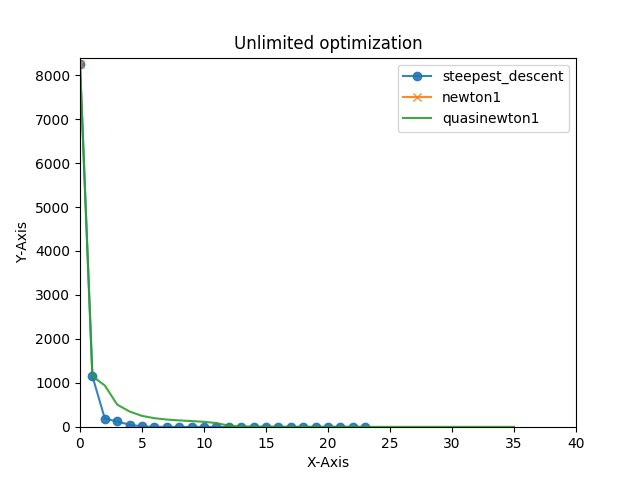
\includegraphics[width=12cm]{./graph1.png}
  \caption{探索アルゴリズム比較}
\end{figure}

次に1つのデータを選び、勾配ベクトルの大きさがある程度
小さくなったあと、最急降下法が生成する点列の2次元平面
におけるプロットを作成する\\

$Q,c$の値は上と同じとする。

結果は以下のようになる
探索終了から10遷移分をプロットしている


\begin{figure}[H]
  \centering
  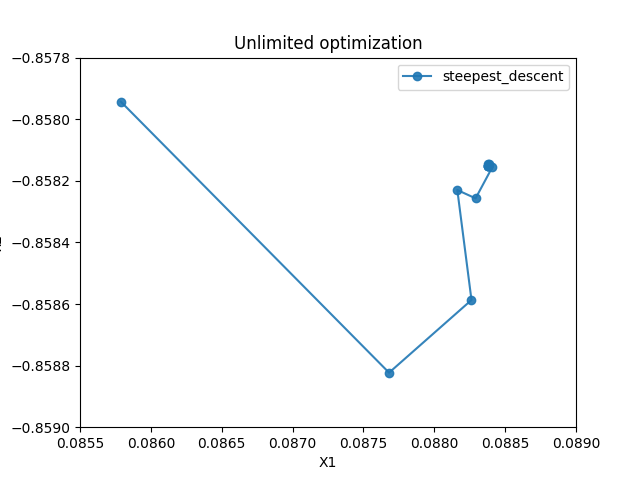
\includegraphics[width=12cm]{./graph3.png}
  \caption{最急降下法が生成した二次元配列}
\end{figure}

\subsubsection{関数が凸関数であるかの吟味}
ある区間で定義された実数値関数 $f$ で、区間内の任意の 2 点 $x$ , $y$ と開区間 (0, 1) 内の任意の $t$ に対して

$$
f(tx + (1 - t)y) \leq tf(x) + (1 - t)f(y)
$$

を満たすものをいう。
ここで

図1からf(x)の値は降下を続け、
また
図2から$(x_1, x_2)$はジグザグと進みながらもその移動距離を小さくしている
すなわち$\nabla f(x)$が収束していっていることがわかり
関数f(x)は凸関数であると言える

\subsection{関数$f(x) = {\Sigma}^{4}_{i=0}{\Sigma}^{4}_{j=0} a_{ij} x^{i}_{1} x^{j}_{2}$に関して}
\subsubsection{ニュートン法、準ニュートン法の収束について}
結果よりニュートン法の収束が速いと言える。
準ニュートン法はBFGS公式によりヘッセ行列${\nabla}^2 f(x)$を近似している。
これによりヘッセ行列${\nabla}^2 f(x)$に逆行列が存在しないことによりこれ以上
探索方向を生成できなくなってしまうというニュートン法の短所を補っている
このからも準ニュートン法はニュートン法の派生であって純粋なニュートン法には
かなわないと推測できた。

\subsubsection{ニュートン法、準ニュートン法が生成した点列の収束先はどのような点になっているか}
ニュートン法においてはニュートン法の局所的2次収束性により
$||x_{k+1} - x^{\ast}|| \leq \Upsilon ||x_{k} - x^{\ast}||$  
が成り立つと言える。ただし$\Upsilon$ は定数である。


またニュートン法、準ニュートン法の収束先については結果より
凸関数であればその頂点部であると考察される。

\section{まとめ}
今回の実験を通して無制約最小化問題の理論をより実践的な理解を
することができたと言える。ニュートン法、準ニュートン法、
そして最急降下法それぞれの式の意味が今回の実験結果を
通して白日のもととなったのだ。
自分は以前東大のGPU貸し出しの応募に受かり
lstmで株式予想や翻訳、cnnで画像認識などをやったこと
があったが最小化問題として共通するところがあり
勉強になったと言える。 

\begin{thebibliography}{9}
  \bibitem{0} 工学基礎 最適化とその応用・矢部博
\end{thebibliography}

\section{コード}
コードは以下のようになった

\lstinputlisting[caption = steepest\_descent.cpp ,label = program2]{4617043_steepest_descent.cpp}
\lstinputlisting[caption = newton1.cpp           ,label = program2]{4617043_newton1.cpp}
\lstinputlisting[caption = newton2.cpp           ,label = program2]{4617043_newton2.cpp}
\lstinputlisting[caption = quasinewton1.cpp      ,label = program2]{4617043_quasinewton1.cpp}
\lstinputlisting[caption = quasinewton2.cpp      ,label = program2]{4617043_quasinewton2.cpp}



\end{document}
